\chapter{Just trying...}

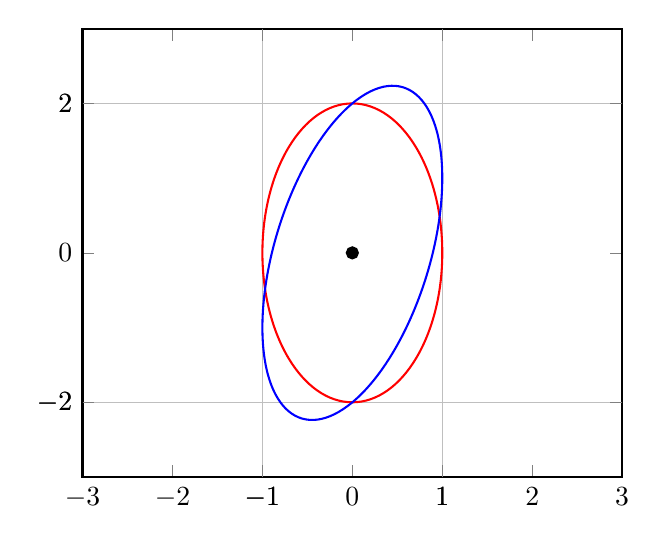
\begin{tikzpicture}
    \begin{axis}[
        xmin=-3,   xmax=3,
        ymin=-3,   ymax=3,
        extra x ticks={-1,1},
        extra y ticks={-2,2},
        extra tick style={grid=major},
    ]
        \draw[red] \pgfextra{
          \pgfpathellipse{\pgfplotspointaxisxy{0}{0}}
            {\pgfplotspointaxisdirectionxy{1}{0}}
            {\pgfplotspointaxisdirectionxy{0}{2}}
          % see also the documentation of 
          % 'axis direction cs' which
          % allows a simpler way to draw this ellipse
        };
        \draw[blue] \pgfextra{
          \pgfpathellipse{\pgfplotspointaxisxy{0}{0}}
            {\pgfplotspointaxisdirectionxy{1}{1}}
            {\pgfplotspointaxisdirectionxy{0}{2}}
        };
        \addplot [only marks,mark=*] coordinates { (0,0) };
    \end{axis}
    \end{tikzpicture}

  
  
  \begin{equation}
      x\in\mathbb{R}^{n}
  \end{equation}

  \begin{figure}[h]
    \centering
    \includegraphics[width=8cm]{pdfs/modperf/antidebug_setunhandledexceptionfilter.bson-pr.pdf}
    \caption{Example of a parametric plot ($\sin (x), \cos(x), x$)}
    \label{fig:something}
  \end{figure}

  \begin{figure}
    \centering
    \begin{subfigure}{.33\textwidth}
      \centering
      \includegraphics[width=.8\linewidth]{pdfs/modperf/antidebug_setunhandledexceptionfilter.bson-pr.pdf}
      \caption{1a}
      \label{fig:sfig1}
    \end{subfigure}%
    \begin{subfigure}{.33\textwidth}
      \centering
      \includegraphics[width=.8\linewidth]{pdfs/modperf/antidebug_setunhandledexceptionfilter.bson-roc.pdf}
      \caption{1b}
      \label{fig:sfig2}
    \end{subfigure}
    \begin{subfigure}{.33\textwidth}
        \centering
        \includegraphics[width=.8\linewidth]{pdfs/modperf/antidebug_setunhandledexceptionfilter.bson-roclog.pdf}
        \caption{1c}
        \label{fig:sfig3}
    \end{subfigure}
    \caption{plots of....}
    \label{fig:fig}
\end{figure}


\begin{table}[h]
  \centering
  \caption{This is first table}
  \begin{tabular}{@{}llr@{}} \toprule
      \multicolumn{2}{c}{Item} \\ \cmidrule(r){1-2}
      Animal & Description & Price (\$)\\ \midrule
      Gnat & per gram & 13.65 \\
      & each & 0.01 \\
      Gnu & stuffed & 92.50 \\
      Emu & stuffed & 33.33 \\
      Armadillo & frozen & 8.99 \\ \bottomrule
  \end{tabular}        
\end{table}

\begin{algorithm}
  \caption{Dependency Graph Assembly}\label{algo:AKP13_command_dependency_graph_assembly}
  \begin{algorithmic}[1]
      \Procedure{MyProcedure}{}
      \State $\textit{stringlen} \gets \text{length of }\textit{string}$
      \State $i \gets \textit{patlen}$
      \If {$i > \textit{stringlen}$} \Return false
      \EndIf
      \State $j \gets \textit{patlen}$
      \If {$\textit{string}(i) = \textit{path}(j)$}
      \State $j \gets j-1$.
      \State $i \gets i-1$.
      \State \textbf{goto} \emph{loop}.
      \State \textbf{close};
      \EndIf
      \State $i \gets i+\max(\textit{delta}_1(\textit{string}(i)),\textit{delta}_2(j))$.
      \State \textbf{goto} \emph{top}.
      \EndProcedure
  \end{algorithmic}
\end{algorithm}

\tikzset{every picture/.style={line width=0.75pt}} %set default line width to 0.75pt        

\begin{center}
    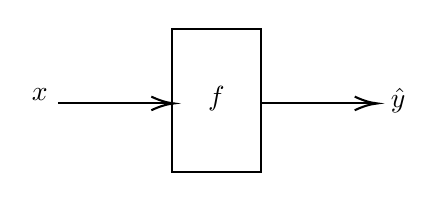
\begin{tikzpicture}[x=0.75pt,y=0.75pt,yscale=-1,xscale=1]
        %uncomment if require: \path (0,269); %set diagram left start at 0, and has height of 269
        
        %Shape: Rectangle [id:dp8386354950784081] 
        \draw   (258,67) -- (301,67) -- (301,136) -- (258,136) -- cycle ;
        %Straight Lines [id:da9088407411543793] 
        \draw    (203,103) -- (257,103) ;
        \draw [shift={(259,103)}, rotate = 180] [color={rgb, 255:red, 0; green, 0; blue, 0 }  ][line width=0.75]    (10.93,-3.29) .. controls (6.95,-1.4) and (3.31,-0.3) .. (0,0) .. controls (3.31,0.3) and (6.95,1.4) .. (10.93,3.29)   ;
        %Straight Lines [id:da7684121128470209] 
        \draw    (301,103) -- (355,103) ;
        \draw [shift={(357,103)}, rotate = 180] [color={rgb, 255:red, 0; green, 0; blue, 0 }  ][line width=0.75]    (10.93,-3.29) .. controls (6.95,-1.4) and (3.31,-0.3) .. (0,0) .. controls (3.31,0.3) and (6.95,1.4) .. (10.93,3.29)   ;
        
        % Text Node
        \draw (189,94.4) node [anchor=north west][inner sep=0.75pt]    {$x$};
        % Text Node
        \draw (274,93.4) node [anchor=north west][inner sep=0.75pt]    {$f$};
        % Text Node
        \draw (362,94.4) node [anchor=north west][inner sep=0.75pt]    {$\hat{y}$};
        
        
        \end{tikzpicture}
            
\end{center}